\section{}
Consider the closed-loop feedback system
\begin{figure}[h]
    \centering
    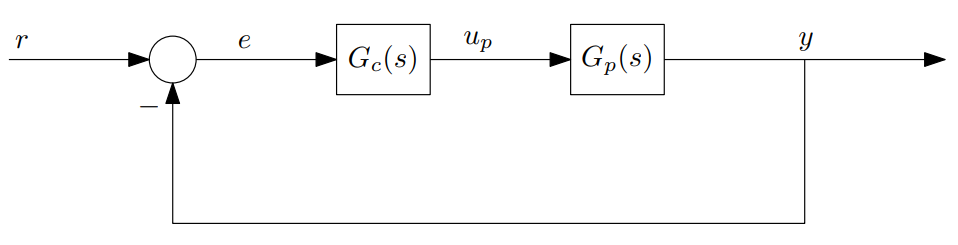
\includegraphics[width=0.8\linewidth]{Questions/Figures/Q2ProblemDiagram.png}
    \caption{Closed-loop feedback system}
    \label{fig:Q2ProblemDiagram}
\end{figure}
with a plant model
\begin{equation*}
    G_p(s) = \frac{1}{s(s+1)(s+5)}
\end{equation*}
and a PID controller of the form
\begin{equation*}
    G_c(s) = k_p + \frac{k_i}{s} + k_d s
\end{equation*}
with gain values of $k_p = 39.42, k_i = 12.81, k_d = 30.32$ obtained by tuning, providing a stable
closed-loop system. 
\begin{enumerate}[label=(\alph*)]
    \item Will this system be able to asymptotically track a reference step $r(t) = 1_{+}(t)$? A ramp
    $r(t) = t$? A sine wave $r(t) = \sin t$? Explain why or why not in each case.
    \item Using Simulink's PID Controller block, simulate the response of the system for each type of
    reference input given in (b). Show the plot of $y$ in each case. Note: in the parameters of this
    block, leave the Filter coefficient ($N$) at its default value of 100.
\end{enumerate}

\subsection{}
From Section 4.4, 
\begin{equation*}
    Y = \frac{G_p G_c}{1 + G_p G_c} R = G_{yr} R
\end{equation*}
For $R_{1} = 1_{+}(t)$, $R_{t} = t$, and $R_{\text{wave}} = \sin t$, $Y$ is, by Matlab,
\begin{verbatim}
clc; clear all; close all;
syms s t;
Gc = 39.42 + 12.81/s + 30.32*s;
Gp = 1/(s*(s+1)*(s+5));
G_yr = Gc*Gp/(1+Gc*Gp);

R1 = laplace(1 + 0*t);
Rt = laplace(t);
Rsin = laplace(sin(t));

Y1 = simplify(G_yr*R1)
Yt = simplify(G_yr*Rt)
Ysin = simplify(G_yr*Rsin)
\end{verbatim}
\begin{align*}
    Y_1 &= \frac{3032 s^2 + 3942 s + 1281}{s(100 s^4 + 600 s^3 + 3532 s^2 + 3942 s + 1281)} \\
    Y_t &= \frac{3032 s^2 + 3942 s + 1281}{s^2(100 s^4 + 600 s^3 + 3532 s^2 + 3942 s + 1281)} \\
    Y_{\text{wave}} &= \frac{3032 s^2 + 3942 s + 1281}{100 s^6 + 600 s^5 + 3632 s^4 + 4542 s^3 + 4813 s^2 + 3942 s + 1281}
\end{align*}
Looking for the roots for $Y_1$, 
\begin{verbatim}
>> vpa(root((s*(100*s^4 + 600*s^3 + 3532*s^2 + 3942*s + 1281)), s))
 
ans =
 
                                                                         0
- 0.64860612459783461771340131819613 - 0.15652180448584118882475979750655i
- 0.64860612459783461771340131819613 + 0.15652180448584118882475979750655i
  - 2.3513938754021653822865986818039 - 4.8213321796848982440561485616617i
  - 2.3513938754021653822865986818039 + 4.8213321796848982440561485616617i
\end{verbatim}
Since all the roots have negative real parts, the system is stable and will be able to asymptotically track a reference step $r(t) = 1_{+}(t)$.

Looking for the roots for $Y_t$,
\begin{verbatim}
>> vpa(root((s^2*(100*s^4 + 600*s^3 + 3532*s^2 + 3942*s + 1281)), s))
 
ans =
 
                                                                         0
                                                                 1.0e-1032
- 0.64860612459783461771340131819613 - 0.15652180448584118882475979750655i
- 0.64860612459783461771340131819613 + 0.15652180448584118882475979750655i
  - 2.3513938754021653822865986818039 + 4.8213321796848982440561485616617i
  - 2.3513938754021653822865986818039 - 4.8213321796848982440561485616617i
\end{verbatim}
Since there is a root with Re$(s) > 0$, the system is unstable and will not be able to asymptotically track a ramp $r(t) = t$.

Looking for the roots for $Y_{\text{wave}}$,
\begin{verbatim}
>> vpa(root((100*s^6 + 600*s^5 + 3632*s^4 + 4542*s^3 + 4813*s^2 + 3942*s + 1281), s))
 
ans =
    
- 0.64860612459783461771340131819613 - 0.15652180448584118882475979750655i
- 0.64860612459783461771340131819613 + 0.15652180448584118882475979750655i
                                                                        -1.0i
                                                                        1.0i
    - 2.3513938754021653822865986818039 - 4.8213321796848982440561485616617i
    - 2.3513938754021653822865986818039 + 4.8213321796848982440561485616617i
\end{verbatim}
Since the system has a root at Re$(s) = 0$, the system is unstable and will not be able to asymptotically track a sine wave $r(t) = \sin t$.

\subsection{}
\begin{figure}[h]
    \centering
    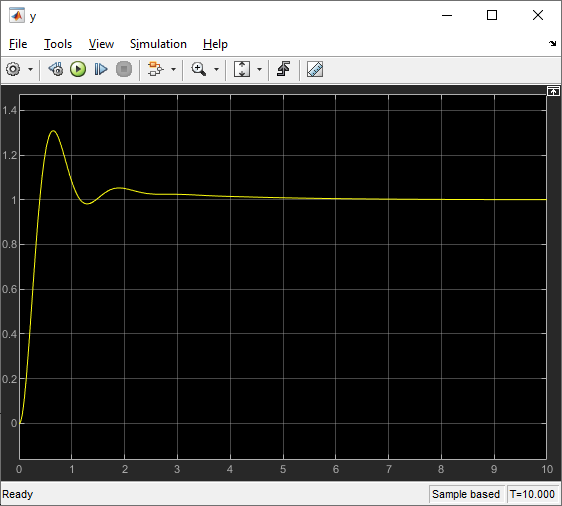
\includegraphics[width=0.5\linewidth]{Questions/Figures/q2plot1.png}
    \caption{Response of $y$ to a step input $r(t) = 1_{+}(t)$}
    \label{fig:q2plot1}
\end{figure}
\begin{figure}[h]
    \centering
    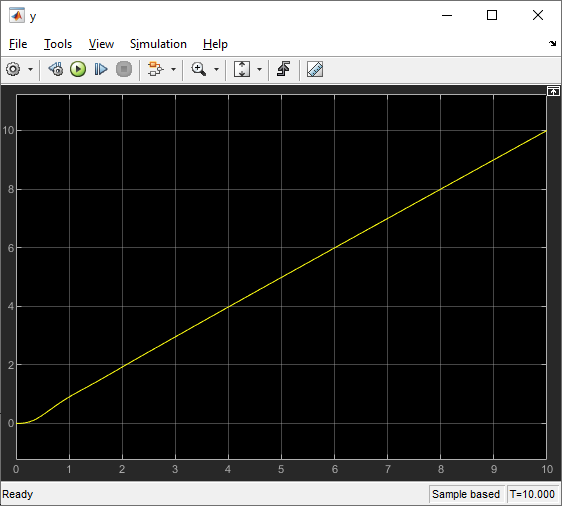
\includegraphics[width=0.5\linewidth]{Questions/Figures/q2plot2.png}
    \caption{Response of $y$ to a ramp input $r(t) = t$}
    \label{fig:q2plot2}
\end{figure}
\begin{figure}[h]
    \centering
    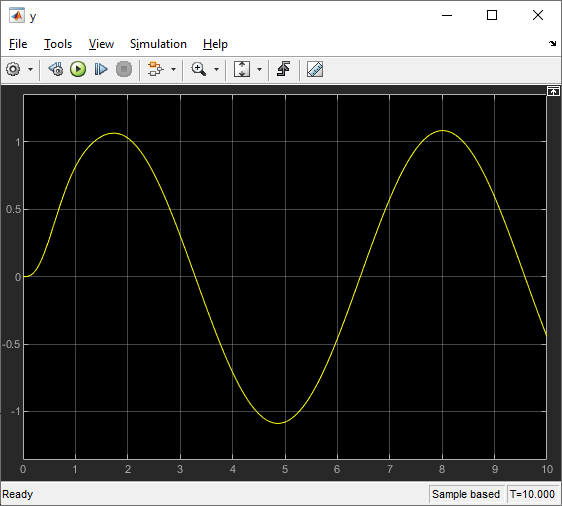
\includegraphics[width=0.5\linewidth]{Questions/Figures/q2plot3.png}
    \caption{Response of $y$ to a sine wave input $r(t) = \sin t$}
    \label{fig:q2plot3}
\end{figure}
